\section{Einführung}

\subsection{Motivation}

% start with something familiar?

\addtocounter{framenumber}{1}
\begin{frame}[standout]
    \LARGE
    Was erwartest du dir \\
    von diesem Workshop?
\end{frame}


\begin{frame}[c]{Situation}
    \Large
    \begin{itemize}[<+(1)->]
        \item Man hat etwas vor
        \item Es kommt etwas dazwischen
        \item Ziel wird vergessen
    \end{itemize}
\end{frame}

\begin{frame}[c]{Ziel des Workshops}
    \Large
    \begin{itemize}[<+(1)->]
        \item Jeder schreibt seine Ziele auf
        \item Jeder macht sich sehr genaue Gedanken
        \item Jeder sucht sich eine Vertrauensperson, um den Fortschritt regelmäßig zu teilen
    \end{itemize}
\end{frame}


% Forschung: 149/267 Teilnehmer
% Zufällig gruppe zugewiesen
% - gruppe 1 hat sich über die Ziele gedanken gemacht
%   rate that goal on the following dimensions: Difficulty, Importance, the
%   extent to which they had the Skills & Resources to accomplish the goal,
%   their Commitment and Motivation to the goal, whether or not they had
%   Pursued this goal before and if so their Prior Success.
% jede gruppe hat auch das getan, was die gruppe davor getan hat

\begin{frame}[c]{Stand der Forschung}
    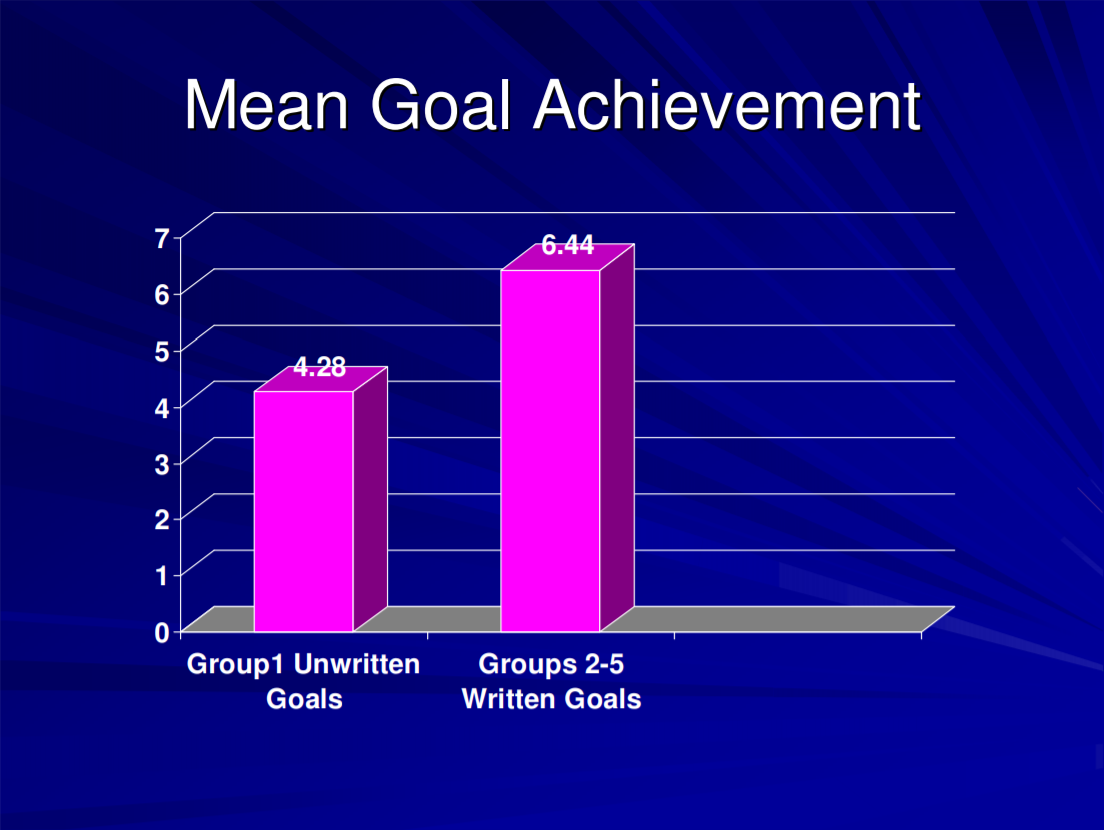
\includegraphics[height=0.8\textheight]{goal_achievement_two} \\
    Nach \cite{better-goals-2} hilft es, seine Ziele aufzuschreiben.
\end{frame}

\begin{frame}[c]{Stand der Forschung II}
    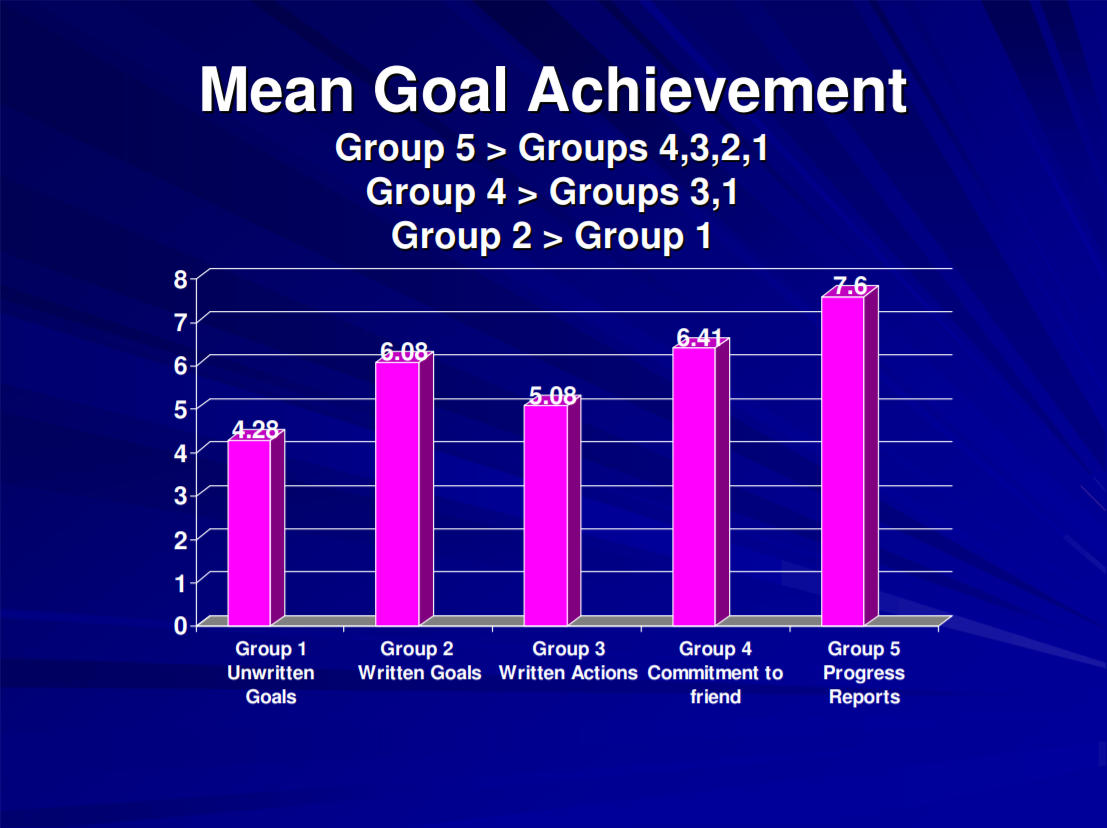
\includegraphics[height=0.8\textheight]{goal_achievement_all} \\
    Außerdem gibt es weitere helfende Maßnahmen \cite{better-goals-2}.
\end{frame}



\subsection{Ablauf}


\begin{frame}[c]{Ablauf}
    \begin{itemize}[<+(1)->]
        \item Ich gebe ein Thema/Aufgabe vor
        \item Erkläre, warum man das machen will
        \item Was die Erfolgskriterien sind
        \item Jeder bearbeitet die Aufgabe
        \item Jeder der will, teilt seine Ergebnisse/Erfolge
        \item Repeat
    \end{itemize}
\end{frame}


\begin{frame}[c]{Vorbereitung}
    \begin{itemize}[<+(1)->]
        \item Papier und Stift bereitlegen
        \item Platzhalter für Ideen anlegen
        \item Platz für Markierungen lassen
        \item (Evtl: Ausführung \cite{longtermplans-post} oder PDF \cite{longtermplans-pdf} in einem Tab öffnen)
    \end{itemize}
    \pause
    PDF: \url{https://github.com/fkarg/things-to-talk-about/blob/master/longtermplans/main_handout.pdf}
\end{frame}


\begin{frame}[c]{Agenda}
    \Large
    \begin{itemize}[<+(1)->]
        \item Inhalt: Hängt von euch ab!
        \item Format: Interaktiv!
        \item Immer: Listen schreiben!
    \end{itemize}
\end{frame}


\begin{frame}[c]{Themen}
    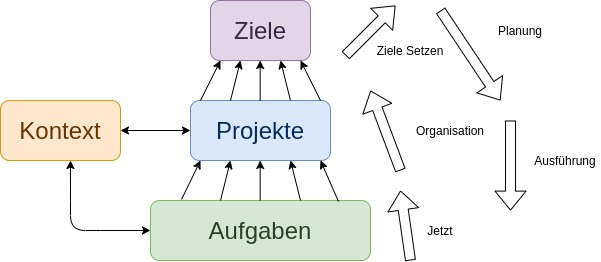
\includegraphics[width=\textwidth]{Ziele_Aufgaben}
\end{frame}


\begin{frame}[c]{Thema: Jetzt}
    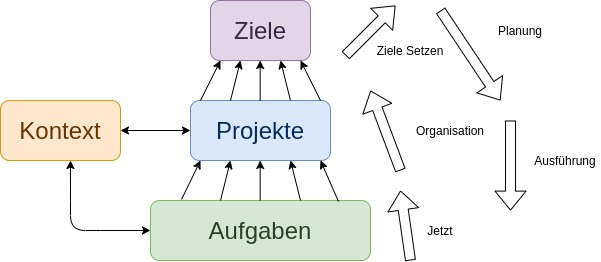
\includegraphics[width=\textwidth]{Ziele_Aufgaben}
\end{frame}





